\section{MATERIALS AND METHODS}

\subsection{Artificial Dataset Synthesis}
\label{subsec:synth_dataset}

The strategy of generating training data synthetically, or augmenting real
imagery with synthetic elements, is well established in computer vision
research where labelled data are scarce or impractical to collect at scale.
This approach enables fine-grained control over scene parameters---including
geometry, illumination, and camera pose---and has been successfully applied to
tasks ranging from smoke detection to fiducial marker
localisation~\cite{BlenderSmoke,BlurFiducial,ObjetoSintetico}. Fully
photorealistic scenes can be rendered with configurable lighting direction,
colour temperature, and intensity, and may include shadows and other
environmental effects, producing synthetic datasets whose utility has been
demonstrated in related works~\cite{TurbineBlur,BlenderMapa}.

Following this paradigm, a synthetic image bank was generated in Blender using
a photorealistic water surface model that simulates quiescent fluid behaviour
representative of enclosed water bodies such as reservoirs, lakes, and large
dams. Representative RGB samples are shown in Fig.~\ref{fig:rgb}. The wave
geometry was synthesised using a time-varying three-dimensional noise algorithm
to model surface undulation~\cite{OndaR,OndaDeep}. Solar illumination was
simulated with Blender's built-in sun lamp, which models a directional light
source with spectrally configurable colour and intensity, thereby capturing the
chromatic variation in sunlight across different times of day and atmospheric
conditions.

Images were rendered at 21 discrete altitude levels spanning 50 to 800~cm
--- specifically 50, 60, 70, 80, 90, 100, 120, 140, 160, 180, 200, 240, 280,
320, 360, 400, 480, 560, 640, 720, and 800~cm --- with 9{,}000 raw images per
level, yielding a total of 189{,}000 rendered images before preprocessing.

\begin{figure}[!h]
    \centering
    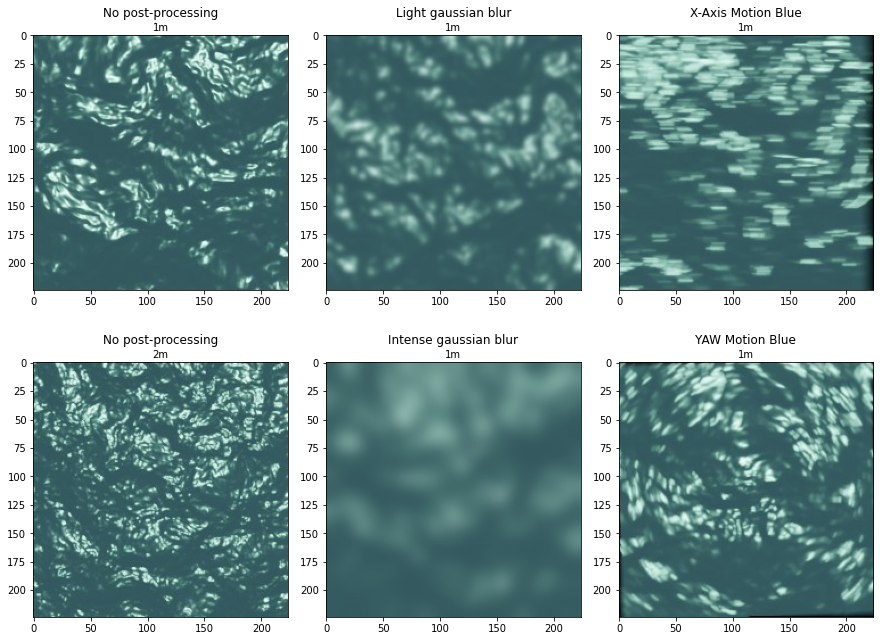
\includegraphics[width=15cm]{Images/rgb.png}
    \caption{Synthetic RGB images rendered at representative altitude levels.
             Labels describe each sample's configuration.}
    \label{fig:rgb}
\end{figure}

% ──────────────────────────────────────────
\subsubsection{Image Preprocessing Pipeline}
\label{subsubsec:synth_preproc}

Following rendering, a three-step preprocessing pipeline was applied offline
to each image using a C++ routine built on OpenCV, as diagrammed in
Fig.~\ref{fig:flow}.

\begin{enumerate}

    \item \textbf{Motion blur augmentation.} Blur was applied in three
    directions: single-axis (simulating forward flight), diagonal (simulating
    oblique movement), and rotational (simulating yaw movement). This captures
    the range of apparent image motion induced by a quadrotor in
    operation~\cite{YawBlur,MotionBlur,SynthBlurDeblur}.

    \item \textbf{Gaussian blur augmentation.} A Gaussian kernel was applied
    to emulate optical defocus and condensation artefacts common on camera
    lenses in humid environments.

    \item \textbf{HSV Value channel extraction.} Each RGB image was converted
    to the HSV color space and only the V channel was retained. As defined by
    $V = \max(R,\,G,\,B)$, the Value channel preserves specular highlights,
    which correlate with surface texture and thus encode altitude-dependent
    information, while discarding hue and saturation. This step reduces the
    network's sensitivity to color variations arising from biome-specific
    water coloration, suspended sediment, and algal content~\cite{ColorTurb},
    and increases robustness to chromatic differences between the synthetic
    and real domains. Fig.~\ref{fig:rgb_vs_v} illustrates the contrast between
    the RGB input and the extracted V channel at three altitude levels.

\end{enumerate}

For steps 1 and 2, kernel parameters were calibrated by fitting a Gaussian distribution to color statistics extracted from real-world images of a coastal site, ensuring that the simulated distortions are representative of field conditions.

This offline approach was preferred over runtime data augmentation in Keras for two reasons: it allows a precisely controlled and documented distribution of distortion types across the training set, and it avoids the cold posterior effect associated with insufficient augmentation diversity in large-scale training~\cite{BadData}. The resulting distribution of distortion configurations per altitude set is summarized in Table~\ref{tab:preproc_dist}. Examples of preprocessed images without any blur are shown in Fig.~\ref{fig:v}, and examples with varying levels of motion blur are shown in Fig.~\ref{fig:dist}.

\begin{figure}[h]
    \centering
    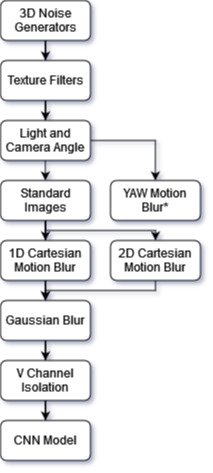
\includegraphics[width=7cm]{Images/flow.jpg}
    \caption{Preprocessing pipeline flowchart. For real-world images, the
             pipeline begins at the Gaussian blur stage.}
    \label{fig:flow}
\end{figure}

\begin{table}[htbp]
    \caption{Preprocessing distribution for each altitude set of synthetically
             generated images. Each cell indicates the number of images per
             distortion configuration.}
    \begin{center}
        \begin{tabular}{|l|c|c|}
        \hline
        \textbf{Distortion class (all 21 altitude sets)}
            & \textbf{No Gaussian blur}
            & \textbf{Gaussian blur} \\
        \hline
        No motion blur          & 1{,}500 & 1{,}500 \\
        \hline
        Single-axis motion blur & 1{,}500 & 1{,}500 \\
        \hline
        Diagonal motion blur    & 1{,}500 & 1{,}500 \\
        \hline
        \end{tabular}
    \label{tab:preproc_dist}
    \end{center}
\end{table}

\begin{figure}[!h]
    \centering
    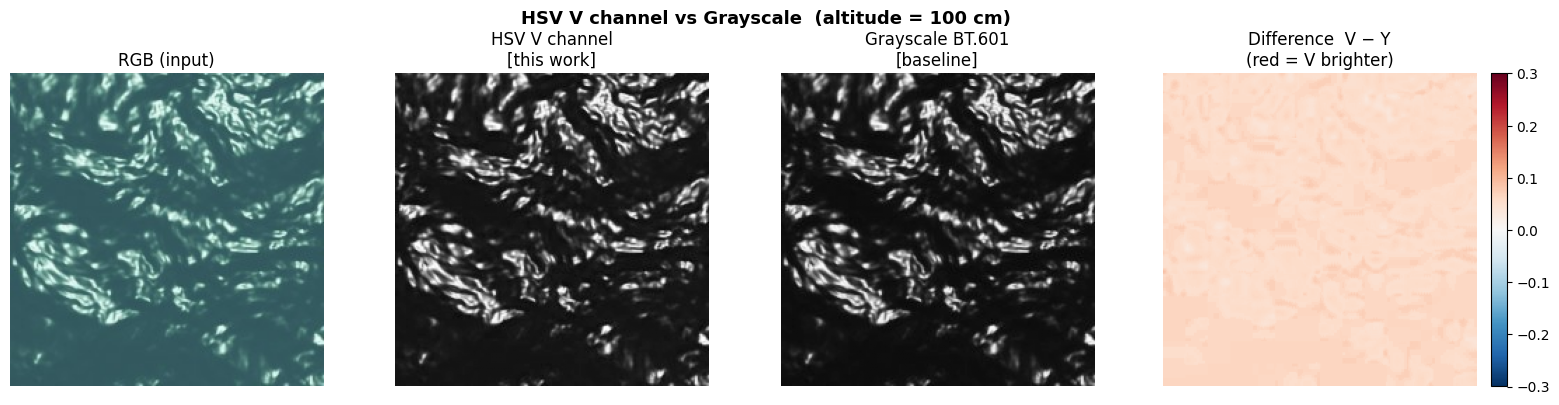
\includegraphics[width=\textwidth]{Images/01_rgb_vs_value_channel_comparison.png}
    \caption{Side-by-side comparison of a synthetic RGB image (left) and the
             corresponding HSV Value channel image (right) at 100~cm altitude.
             Discarding hue and saturation eliminates colour cast from the
             water surface while retaining the specular texture structure.}
    \label{fig:rgb_vs_v}
\end{figure}

\begin{figure}[!h]
    \centering
    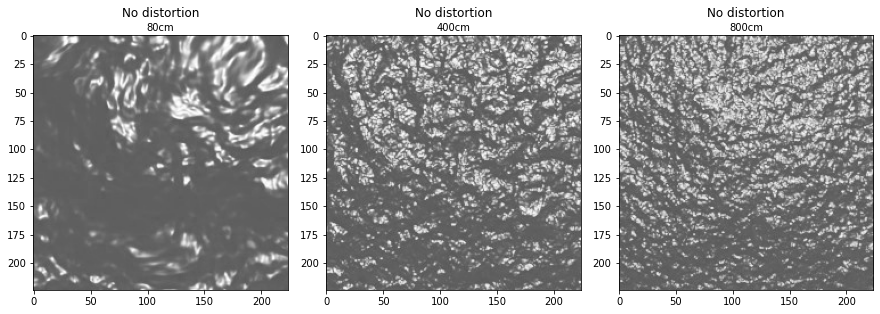
\includegraphics[width=15cm]{Images/samples_std.png}
    \caption{Synthetic Value-channel images at 80, 400, and 800~cm (left to
             right) with no blur applied. The progressive smoothing of surface
             texture with increasing altitude is clearly visible.}
    \label{fig:v}
\end{figure}

\begin{figure}[!h]
    \centering
    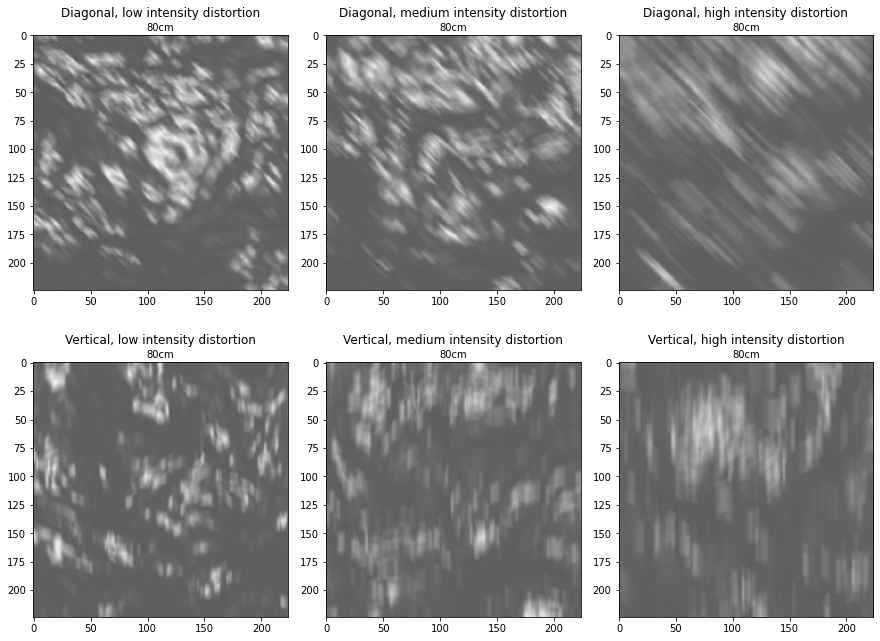
\includegraphics[width=15cm]{Images/samples_motion.png}
    \caption{Synthetic Value-channel images at 80~cm with motion blur at
             different intensities. Blur direction and magnitude increase from
             left to right.}
    \label{fig:dist}
\end{figure}

\subsection{Computational Platform and Training Infrastructure}
\label{subsec:platform}

Blender rendering of the synthetic dataset was carried out on a workstation equipped with an AMD Ryzen\textsuperscript{TM} 1600 six-core processor overclocked to 3.8~GHz, an NVIDIA GeForce GTX~970 GPU (4~GB GDDR5; base clock 1{,}165~MHz, boost 1{,}317~MHz; NVIDIA Corp., Santa Clara, CA, USA), and 16~GB of DDR4-2800 RAM (2$\times$8~GB; Micron Technology Inc., Boise, ID, USA). The operating system was Ubuntu 18.04 LTS with NVIDIA driver version 481.1. Initial CNN experiments were conducted on this same platform under Keras~2.4.3 / TensorFlow~2.3.1.

Subsequent training runs were migrated to a Google Colab environment with an NVIDIA L4 GPU (24~GB GDDR6; high-memory instance) running TensorFlow~2.19.0 and Python~3.10. This transition provided sufficient GPU memory for the ResNet50-based architectures and enabled a reproducible cloud execution environment. All training runs used a fixed global random seed (\texttt{SEED = 42}) applied to NumPy, TensorFlow, and the Python hash environment.

\subsection{Feature Engineering}
\subsubsection{Image Input and Value Channel Extraction}
\label{subsubsec:vchannel}

Each input image is first resized to $224 \times 224$ pixels using area interpolation (\texttt{INTER\_AREA}), which minimizes aliasing during downscaling. The RGB image is then converted to the HSV color space and the Value channel is isolated, after which pixel intensities are normalized to the range $[0, 1]$. As discussed in Section~\ref{subsec:synth_dataset}, retaining $V$ rather than a weighted luminance (e.g.\ ITU-R BT.601) preserves specular highlight peaks that carry altitude-correlated texture information, while removing color variation unrelated to height.

Fig.~\ref{fig:batch_samples} shows four training-set images with their corresponding standardized altitude labels, illustrating the visual diversity of the training distribution after preprocessing.

\begin{figure}[!h]
    \centering
    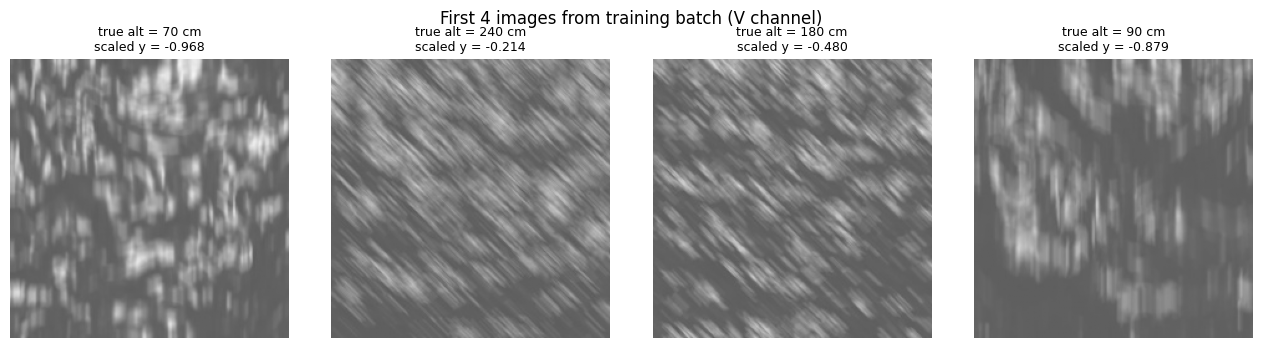
\includegraphics[width=\textwidth]{Images/04_training_batch_sample_grid.png}
    \caption{Four Value-channel images drawn from a single training batch, with
             true altitude labels (cm) and their standardized counterparts.
             The texture density visibly increases with altitude.}
    \label{fig:batch_samples}
\end{figure}

% ─────────────────────────────────────────────────
\subsubsection{Pre-processed Feature Vector}
\label{subsubsec:features}

For the multi-input fusion architectures, a 12-element pre-processed feature vector is extracted from the Value channel alongside the image matrix. The vector encodes pixel statistics, spectral energy distribution, gradient statistics, texture entropy, corner density, and local variance. Feature definitions and their expected monotonic relationship with altitude are summarized in Table~\ref{tab:features}. Each element was chosen in a empirical battery of tests, trying to emulate a weak learning strategy, as seen in systems based on random forest, or more modern tabular models like LightGBM.

\begin{table}[htbp]
    \caption{Pre-processed feature vector: index, name, description, and
             expected trend with \emph{increasing} altitude.
             $\uparrow$~=~increases, $\downarrow$~=~decreases.}
    \begin{center}
        \small
        \begin{tabular}{|c|l|p{7cm}|c|}
        \hline
        \textbf{Idx} & \textbf{Name} & \textbf{Description} & \textbf{Trend} \\
        \hline
        0  & \texttt{mean\_v}
           & Mean pixel intensity of the V channel
           & $\uparrow$ \\
        \hline
        1  & \texttt{std\_v}
           & Standard deviation of V channel
           & $\downarrow$ \\
        \hline
        2  & \texttt{skew\_v}
           & Skewness of intensity distribution
           & $\downarrow$ \\
        \hline
        3  & \texttt{kurt\_v}
           & Kurtosis; glints produce heavy tails at low altitude
           & $\downarrow$ \\
        \hline
        4  & \texttt{fft\_energy\_low}
           & FFT energy fraction in $r < 0.20$ (large-scale / DC)
           & $\downarrow$ \\
        \hline
        5  & \texttt{fft\_energy\_mid}
           & FFT energy in $0.20 \leq r < 0.60$
           & $\uparrow$ \\
        \hline
        6  & \texttt{fft\_energy\_high}
           & FFT energy in $r \geq 0.60$ (fine ripples / capillary waves)
           & $\uparrow$ \\
        \hline
        7  & \texttt{grad\_mean}
           & Mean Sobel gradient magnitude
           & $\uparrow$ \\
        \hline
        8  & \texttt{grad\_std}
           & Standard deviation of Sobel gradient magnitude
           & $\uparrow$ \\
        \hline
        9  & \texttt{entropy}
           & Normalised image entropy over a 32-bin histogram
           & $\uparrow$ \\
        \hline
        10 & \texttt{shi\_tomasi\_count}
           & Shi-Tomasi corner count (glint density proxy)
           & $\uparrow$ \\
        \hline
        11 & \texttt{local\_std\_mean}
           & Mean standard deviation of non-overlapping $8\times8$ blocks
           & $\uparrow$ \\
        \hline
        \end{tabular}
    \label{tab:features}
    \end{center}
\end{table}

\paragraph{FFT (\texttt{fft\_energy}).}The three FFT energy features (indices 4--6) are computed by partitioning the 2D log-magnitude spectrum into concentric radial frequency bands. Defining the normalized radial coordinate $r \in [0,1]$ as the Euclidean distance from the DC component relative to the maximum possible frequency radius, the fractional energy in band $k$ is:

\begin{equation}
    E_k = \frac{\displaystyle\sum_{(u,v)\,\in\,B_k} |\mathcal{F}(u,v)|}
               {\displaystyle\sum_{u,v} |\mathcal{F}(u,v)| + \varepsilon},
    \label{eq:fft_energy}
\end{equation}

\noindent where $B_k$ is the set of frequency components in band $k$ and $\varepsilon$ is a small constant for numerical stability. At low altitudes the surface texture appears coarser, concentrating spectral energy near DC (low band); at high altitudes fine ripple patterns redistribute energy toward higher radial frequencies (high band). Fig.~\ref{fig:fft_bands} confirms this trend empirically on the synthetic dataset, and Fig.~\ref{fig:shi_tomasi} shows the corresponding increase in Shi-Tomasi corner count with altitude.

\begin{figure}[!h]
    \centering
    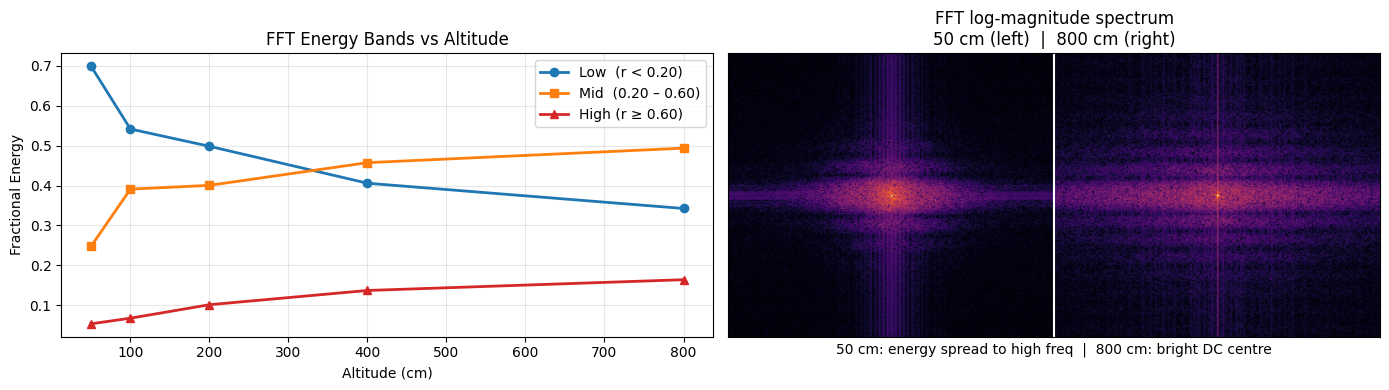
\includegraphics[width=\textwidth]{Images/02_fft_energy_bands_vs_altitude.png}
    \caption{Left: fractional FFT energy in each radial band as a function of
             altitude (average over eight samples per level). As altitude
             increases, energy migrates from the low band to the mid and high
             bands, consistent with the appearance of finer ripple structures
             at greater distances. Right: log-magnitude spectra at 50~cm
             (left half) and 800~cm (right half); the 800~cm spectrum shows a
             broader energy distribution and a brighter DC peak.}
    \label{fig:fft_bands}
\end{figure}

\paragraph{Mean Sobel gradient magnitude (\texttt{grad\_mean}).} The Sobel operator is applied separately along the horizontal and vertical axes of the Value channel using $3\times3$ kernels, and the resulting gradient magnitude map $\|\nabla V\| = \sqrt{G_x^2 + G_y^2}$ is computed at every pixel. The mean of this map measures the average edge strength across the entire image. At low altitudes, the camera resolves large individual wave facets that produce few, well-separated intensity transitions; as altitude increases, a greater number of smaller surface features become simultaneously visible within the field of view, raising the overall density of edges and consequently the mean gradient magnitude.

\paragraph{Standard deviation of Sobel gradient magnitude (\texttt{grad\_std}).}
Computed over the same pixel-wise gradient magnitude map as \texttt{grad\_mean}, the standard deviation captures the spatial variability of edge strength rather than its average level. A low value indicates that gradient magnitudes are uniformly distributed across the image, while a high value reflects the presence of localised high-contrast regions---such as specular glint hotspots or sharp wave crests---surrounded by smoother areas. This feature therefore encodes information about the heterogeneity of the surface texture, which changes with altitude as the spatial distribution of resolvable wave structures evolves.

\paragraph{Normalized image entropy (\texttt{entropy}).} 
A 32-bin histogram of Value channel pixel intensities is constructed over the range $[0, 1]$, and Shannon entropy is computed as $H = -\sum_i p_i \log_2 p_i$, then divided by $\log_2 32$ to normalize it to $[0, 1]$. A small constant $\varepsilon = 10^{-10}$ is added to each bin before the logarithm evaluation to avoid undefined values. High entropy indicates a broad, uniform intensity distribution characteristic of complex, multi-scale surface textures visible at higher altitudes; low entropy indicates a peaked distribution where most pixels share similar brightness values, which occurs close to the surface where large smooth facets dominate the image.

\paragraph{Shi-Tomasi corner count (\texttt{shi\_tomasi\_count}).}
The Shi-Tomasi detector~\cite{ShiTomasi1994} identifies image points at which both eigenvalues of the local structure tensor exceed a quality threshold $\tau$, indicating strong intensity gradients in two independent directions. Applied to the Value channel with a quality level of 0.5 and a minimum inter-corner distance of 24~pixels, the detector returned next to 100 candidate points in 1000 samples. On water surfaces, specular reflection peaks create localized high-gradient regions that satisfy the corner criterion; their count therefore serves as a proxy for glint density. As altitude increases, a greater number of wave facets produce resolvable reflections within the field of view, and the detected corner count increases until it saturates at the detector ceiling.

\begin{figure}[!h]
    \centering
    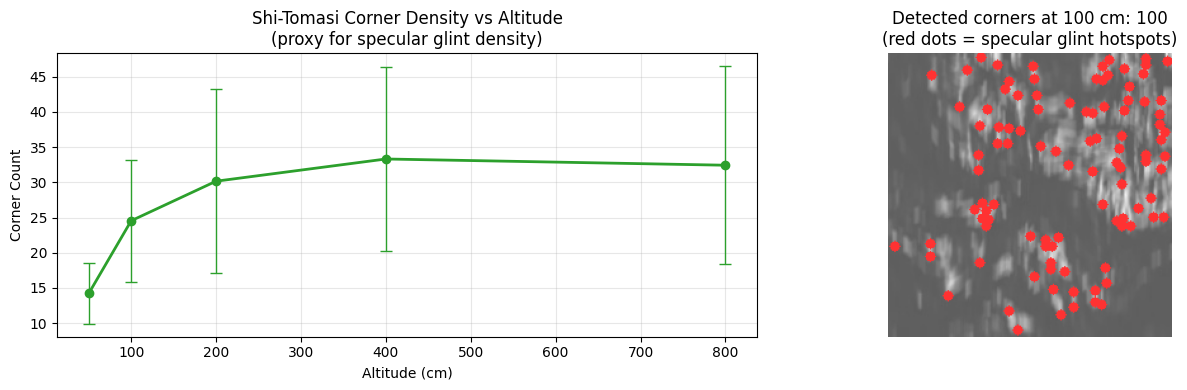
\includegraphics[width=\textwidth]{Images/03_shi_tomasi_corner_density_vs_altitude.png}
    \caption{Shi-Tomasi corner count as a function of altitude.}
    \label{fig:shi_tomasi}
\end{figure}

\paragraph{Mean of $8\times8$ block standard deviations (\texttt{local\_std\_mean}).}
The Value channel image is partitioned into non-overlapping $8\times8$ pixel blocks, and the standard deviation of pixel intensities is computed within each block. The mean of these per-block standard deviations is then taken as a scalar feature. Unlike the global standard deviation of the full image, this measure captures local texture activity at a fixed spatial scale: a block with uniform intensity (smooth water facet) contributes near-zero variance, while a block containing a wave edge or specular glint contributes high variance. The aggregate mean therefore reflects the spatial density of active texture regions, which increases with altitude as more fine-scale surface structures fit within a single $8\times8$ patch.

% ──────────────────────────────────────────────
\subsubsection{Target Normalization and Dataset Split}
\label{subsubsec:data_pipeline}

All ground-truth altitude labels (in centimetres) were standardised prior to
training using a \texttt{StandardScaler} fitted exclusively on the training
partition:

\begin{equation}
    \tilde{y} = \frac{y - \mu_{\text{train}}}{\sigma_{\text{train}}},
    \label{eq:scaler}
\end{equation}

\noindent where $\mu_{\text{train}} = 288.1$~cm and
$\sigma_{\text{train}} = 225.3$~cm are the mean and standard deviation of the training labels. The scaler parameters were saved alongside the model weights and applied in reverse at evaluation to recover metric-scale predictions. Standardization was preferred over linear min-max normalization because it does not bound the output range to $[0,1]$, which is desirable for a
regression head with linear activation.

The synthetic dataset (10{,}517 samples after balancing across altitude levels) was divided into training, validation, and test partitions using a stratified 70/15/15 split, yielding 7{,}365 training, 1{,}574 validation, and 1{,}578 test samples. Stratification was performed by binning altitude labels into 21 equal-width intervals (one per rendered level), ensuring proportional representation of all altitude classes in each
partition.

\subsection{Model Architectures and Training Protocol}
\label{subsec:models}

Four neural network architectures were designed and evaluated within a unified training framework. All models receive the HSV Value channel as their primary image input; two of the four additionally receive a handcrafted 12-element feature vector extracted from the same image. The following subsections describe the shared data pipeline, the individual architectures, and the training procedure.



% ──────────────────────────────────────────────────────
\subsubsection{WaterNet: Custom CNN Baseline}
\label{subsubsec:waternet}

The first architecture, \textit{WaterNet} (\texttt{WaterNet\_CustomCNN}), is a VGG-inspired~\cite{vgg16} convolutional regression network designed for the single-channel Value image. The network consists of four convolutional blocks, each with two consecutive Conv2D layers ($5\times5$ kernels, ReLU activation, same padding) followed by MaxPooling2D (stride 2). Dropout (rate 0.3) is applied after blocks 3 and 4 to regularise the deeper feature maps. A GlobalAveragePooling2D layer replaces the flat-reshape of the original VGG design, producing a 256-dimensional descriptor with far fewer parameters. A three-layer Dense regression head (512 → 256 → 128 units, ReLU, Dropout~0.3) followed by a linear output neuron completes the architecture. An optional \textit{ClampedLinear} layer clips the normalised output to the valid range, enforcing the physical altitude constraint. The full layer sequence is given in Table~\ref{tab:waternet_arch}.

\begin{table}[htbp]
    \caption{\textit{WaterNet} architecture summary.}
    \begin{center}
        \small
        \begin{tabular}{|l|c|r|}
        \hline
        \textbf{Layer (type)} & \textbf{Output shape} & \textbf{Params} \\
        \hline
        image\_input (InputLayer)
            & $(224, 224, 1)$ & 0 \\
        \hline
        conv\_0\_a (Conv2D, $5\times5$, 32)
            & $(224, 224, 32)$ & 832 \\
        conv\_0\_b (Conv2D, $5\times5$, 32)
            & $(224, 224, 32)$ & 25{,}632 \\
        pool\_0 (MaxPooling2D)
            & $(112, 112, 32)$ & 0 \\
        \hline
        conv\_1\_a (Conv2D, $5\times5$, 64)
            & $(112, 112, 64)$ & 51{,}264 \\
        conv\_1\_b (Conv2D, $5\times5$, 64)
            & $(112, 112, 64)$ & 102{,}464 \\
        pool\_1 (MaxPooling2D)
            & $(56, 56, 64)$ & 0 \\
        \hline
        conv\_2\_a (Conv2D, $5\times5$, 128)
            & $(56, 56, 128)$ & 204{,}928 \\
        conv\_2\_b (Conv2D, $5\times5$, 128)
            & $(56, 56, 128)$ & 409{,}728 \\
        pool\_2 (MaxPooling2D) + Dropout(0.3)
            & $(28, 28, 128)$ & 0 \\
        \hline
        conv\_3\_a (Conv2D, $5\times5$, 256)
            & $(28, 28, 256)$ & 819{,}456 \\
        conv\_3\_b (Conv2D, $5\times5$, 256)
            & $(28, 28, 256)$ & 1{,}638{,}656 \\
        pool\_3 (MaxPooling2D) + Dropout(0.3)
            & $(14, 14, 256)$ & 0 \\
        \hline
        gap (GlobalAveragePooling2D)
            & $(256)$ & 0 \\
        \hline
        dense\_0 (Dense, 512) + Dropout(0.3)
            & $(512)$ & 131{,}584 \\
        dense\_1 (Dense, 256) + Dropout(0.3)
            & $(256)$ & 131{,}328 \\
        dense\_2 (Dense, 128) + Dropout(0.3)
            & $(128)$ & 32{,}896 \\
        \hline
        output (Dense, 1, linear)
            & $(1)$ & 129 \\
        \hline
        \multicolumn{2}{|l|}{\textbf{Total trainable parameters}}
            & \textbf{3{,}548{,}897} \\
        \hline
        \end{tabular}
    \label{tab:waternet_arch}
    \end{center}
\end{table}

% ─────────────────────────────────────────────────────────
\subsubsection{WaterNet-Fusion: Multi-Input Late-Fusion Model}
\label{subsubsec:waternet_fusion}

The second architecture, \textit{WaterNet-Fusion} (\texttt{WaterNet\_Fusion}), extends the baseline with a late-fusion branch that ingests the 12-element handcrafted feature vector of Section~\ref{subsubsec:features} in parallel with the image. The \textbf{image branch} is identical to WaterNet up to and including the three Dense layers (512 → 256 → 128 units), each followed by Dropout. The \textbf{feature branch} processes the 12-element vector through two Dense layers (64 → 32 units, ReLU). The 128-dimensional image embedding and the 32-dimensional feature embedding are concatenated (forming a 160-dimensional vector) and passed through a fusion Dense layer (128 units, ReLU) with Dropout, before the linear regression output. A ClampedLinear layer applies the physical constraint to the final prediction.

The \textit{WaterNet-FusionLite} variant (\texttt{WaterNet\_Fusion\_lite}, labelled WN-FusLT in benchmark results) uses a lighter image branch with only three convolutional blocks (32, 64, 128 filters; $3\times3$ kernels) and a single 64-unit embedding Dense layer, fusing a 64-dimensional image embedding with the 32-dimensional feature embedding. This reduces the total parameter count by more than ten-fold relative to WaterNet-Fusion, providing a reference for the accuracy-versus-complexity trade-off. The architecture is presented at Table \ref{tab:wn_fuslite_arch}.

\begin{table}[htbp]
    \caption{\textit{WaterNet-FusionLite} architecture summary.}
    \begin{center}
        \small
        \begin{tabular}{|l|c|r|}
        \hline
        \textbf{Layer (type)}
            & \textbf{Output shape}
            & \textbf{Params} \\
        \hline
        \multicolumn{3}{|l|}{\textit{Image branch}} \\
        \hline
        image\_input (InputLayer)
            & $(224, 224, 1)$ & 0 \\
        \hline
        img\_conv0\_a (Conv2D, $3\times3$, 32)
            & $(224, 224, 32)$ & 320 \\
        img\_conv0\_b (Conv2D, $3\times3$, 32)
            & $(224, 224, 32)$ & 9{,}248 \\
        img\_pool0 (MaxPooling2D)
            & $(112, 112, 32)$ & 0 \\
        \hline
        img\_conv1\_a (Conv2D, $3\times3$, 64)
            & $(112, 112, 64)$ & 18{,}496 \\
        img\_conv1\_b (Conv2D, $3\times3$, 64)
            & $(112, 112, 64)$ & 36{,}928 \\
        img\_pool1 (MaxPooling2D)
            & $(56, 56, 64)$ & 0 \\
        \hline
        img\_conv2\_a (Conv2D, $3\times3$, 128)
            & $(56, 56, 128)$ & 73{,}856 \\
        img\_conv2\_b (Conv2D, $3\times3$, 128)
            & $(56, 56, 128)$ & 147{,}584 \\
        img\_pool2 (MaxPooling2D)
            & $(28, 28, 128)$ & 0 \\
        \hline
        img\_gap (GlobalAveragePooling2D)
            & $(128)$ & 0 \\
        img\_embedding (Dense, 64)
            & $(64)$ & 8{,}256 \\
        \hline
        \multicolumn{3}{|l|}{\textit{Feature branch}} \\
        \hline
        feature\_input (InputLayer)
            & $(12)$ & 0 \\
        feat\_dense0 (Dense, 64)
            & $(64)$ & 832 \\
        feat\_dense1 (Dense, 32)
            & $(32)$ & 2{,}080 \\
        \hline
        \multicolumn{3}{|l|}{\textit{Fusion head}} \\
        \hline
        fusion (Concatenate)
            & $(96)$ & 0 \\
        fusion\_dense (Dense, 128)
            & $(128)$ & 12{,}416 \\
        fusion\_dropout (Dropout)
            & $(128)$ & 0 \\
        output (Dense, 1, linear)
            & $(1)$ & 129 \\
        \hline
        \multicolumn{2}{|l|}{\textbf{Total trainable parameters}}
            & \textbf{310{,}145} \\
        \hline
        \end{tabular}
    \label{tab:wn_fuslite_arch}
    \end{center}
\end{table}

% ──────────────────────────────────────────────────────
\subsubsection{ResNet50 Transfer Learning Baseline}
\label{subsubsec:resnet50}

The third architecture, \textit{WaterNet-ResNet50} (\texttt{WaterNet\_ResNet50}), replaces the custom backbone with a ResNet50~\cite{resnet50} pretrained on ImageNet~\cite{imagenet}. Because the network expects three-channel input and the Value channel is single-channel, the input tensor is expanded by concatenating the channel with itself twice (channel replication):

\begin{equation}
    \mathbf{x}_{3\text{ch}} =
        \bigl[\,V \,\|\, V \,\|\, V\,\bigr] \in \mathbb{R}^{224\times224\times3}.
    \label{eq:channel_rep}
\end{equation}

\noindent The replicated tensor is then processed by \texttt{resnet50.preprocess\_input}, which applies ImageNet zero-centering statistics. The backbone proceeds the same way as in a three channel input.

A two-stage fine-tuning protocol was employed. In \textbf{Stage~1}, the entire ResNet50 backbone was frozen (23{,}587{,}712 non-trainable parameters) and only the regression head was optimized; 557{,}569 parameters were trainable. In \textbf{Stage~2}, the top residual macro-block (\texttt{conv5\_x}) was selectively unfrozen and retrained at a reduced learning rate of $10^{-5}$, while BatchNorm layers were kept in inference mode to preserve the running statistics accumulated during ImageNet pretraining. The full model contains 24{,}145{,}281 parameters in total (92.11~MB).

\begin{table}[htbp]
    \caption{\textit{WaterNet-ResNet50} architecture summary.}
    \begin{center}
        \small
        \begin{tabular}{|l|c|r|}
        \hline
        \textbf{Layer (type)} & \textbf{Output shape} & \textbf{Params} \\
        \hline
        \multicolumn{3}{|l|}{\textit{Input and channel replication}} \\
        \hline
        image\_input (InputLayer)
            & $(224, 224, 1)$ & 0 \\
        channel\_replicate (Concatenate)
            & $(224, 224, 3)$ & 0 \\
        \hline
        \multicolumn{3}{|l|}{\textit{Backbone}} \\
        \hline
        resnet50 (Functional)
            & $(7, 7, 2048)$ & 23{,}587{,}712 \\
        \hline
        \multicolumn{3}{|l|}{\textit{Regression head}} \\
        \hline
        gap (GlobalAveragePooling2D)
            & $(2048)$ & 0 \\
        dense\_0 (Dense, 256) + Dropout
            & $(256)$ & 524{,}544 \\
        dense\_1 (Dense, 128) + Dropout
            & $(128)$ & 32{,}896 \\
        output (Dense, 1, linear)
            & $(1)$ & 129 \\
        \hline
        \multicolumn{2}{|l|}{\textbf{Trainable parameters (Stage~1)}}
            & \textbf{557{,}569} \\
        \hline
        \multicolumn{2}{|l|}{Non-trainable parameters (backbone)}
            & 23{,}587{,}712 \\
        \hline
        \end{tabular}
    \label{tab:resnet50_arch}
    \end{center}
\end{table}

\subsubsection{ResNet50-Fusion: Multi-Input ResNet50 Model}
\label{subsubsec:resnet50_fusion}

The fourth architecture, \textit{WaterNet-ResNet50-Fusion}
(\texttt{WaterNet\_ResNet50\_MultiInput}, labeled RN50-Fus), applies the late-fusion strategy of Section~\ref{subsubsec:waternet_fusion} to the ResNet50 backbone. The \textbf{image branch} uses channel replication, \texttt{resnet50.preprocess\_input}, the frozen ResNet50 backbone, and a 128-unit Dense embedding. The \textbf{feature branch} processes the 12-element vector through two Dense layers (64 → 32 units, ReLU). The 128-dimensional image embedding and 32-dimensional feature embedding are concatenated (160-dimensional fusion vector), passed through a 128-unit fusion Dense layer with Dropout, and fed to the linear output. The model totals 23{,}873{,}633 parameters (91.07~MB), with 285{,}921 trainable in Stage~1.

\begin{table}[htbp]
    \caption{\textit{WaterNet-ResNet50-Fusion} architecture summary.}
    \begin{center}
        \small
        \begin{tabular}{|l|c|r|}
        \hline
        \textbf{Layer (type)} & \textbf{Output shape} & \textbf{Params} \\
        \hline
        \multicolumn{3}{|l|}{\textit{Image branch}} \\
        \hline
        image\_input (InputLayer)
            & $(224, 224, 1)$ & 0 \\
        channel\_replicate (Concatenate)
            & $(224, 224, 3)$ & 0 \\
        resnet50 (Functional)
            & $(7, 7, 2048)$ & 23{,}587{,}712 \\
        img\_gap (GlobalAveragePooling2D)
            & $(2048)$ & 0 \\
        img\_embedding (Dense, 128)
            & $(128)$ & 262{,}272 \\
        \hline
        \multicolumn{3}{|l|}{\textit{Feature branch}} \\
        \hline
        feature\_input (InputLayer)
            & $(12)$ & 0 \\
        feat\_dense0 (Dense, 64)
            & $(64)$ & 832 \\
        feat\_dense1 (Dense, 32)
            & $(32)$ & 2{,}080 \\
        \hline
        \multicolumn{3}{|l|}{\textit{Fusion head}} \\
        \hline
        fusion (Concatenate)
            & $(160)$ & 0 \\
        fusion\_dense (Dense, 128)
            & $(128)$ & 20{,}608 \\
        fusion\_dropout (Dropout)
            & $(128)$ & 0 \\
        output (Dense, 1, linear)
            & $(1)$ & 129 \\
        \hline
        \multicolumn{2}{|l|}{\textbf{Trainable parameters (Stage~1)}}
            & \textbf{285{,}921} \\
        \hline
        \multicolumn{2}{|l|}{Non-trainable parameters (backbone)}
            & 23{,}587{,}712 \\
        \hline
        \end{tabular}
    \label{tab:rn50_fusion_arch}
    \end{center}
\end{table}

A consolidated overview of all four architectures is provided in
Table~\ref{tab:model_summary}.

\begin{table}[htbp]
    \caption{Summary of the four model architectures evaluated. Trainable
             parameters refer to Stage~1 (head-only training) for the
             ResNet50-based models; all parameters are trainable for the
             custom-backbone models.}
    \begin{center}
        \begin{tabular}{|l|l|c|r|r|}
        \hline
        \textbf{Model} & \textbf{Backbone} & \textbf{Feature} &
        \textbf{Total params} & \textbf{Trainable (S1)} \\
        \hline
        WaterNet   & Custom CNN (VGG-style) & No  &  3{,}548{,}897 &  3{,}548{,}897 \\
        \hline
        WN-FusLT   & WaterNet      & Yes &    310{,}145   &    310{,}145   \\
        \hline
        ResNet50   & ResNet50 (ImageNet)    & No  & 24{,}145{,}281 &    557{,}569   \\
        \hline
        RN50-Fus   & ResNet50 (ImageNet)    & Yes & 23{,}873{,}633 &    285{,}921   \\
        \hline
        \end{tabular}
    \label{tab:model_summary}
    \end{center}
\end{table}

% ───────────────────────────────────────────
\subsubsection{Loss Function and Optimizer}
\label{subsubsec:loss_optim}

All models were compiled with the Huber loss:

\begin{equation}
    L_\delta(y,\hat{y}) =
    \begin{cases}
        \dfrac{1}{2}(y - \hat{y})^2
            & \text{if } |y - \hat{y}| \leq \delta, \\[8pt]
        \delta\!\left(|y - \hat{y}| - \dfrac{\delta}{2}\right)
            & \text{otherwise,}
    \end{cases}
    \label{eq:huber}
\end{equation}

\noindent with $\delta = 1.0$ (in normalized target units). The Huber loss provides quadratic gradients near zero error (as in MSE) while remaining linearly bounded for large residuals (as in MAE), which is desirable given the presence of challenging frames (specular glare and two types of blurring) in the dataset.

The AdamW optimizer was used for all models, with initial learning rate $\eta = 10^{-3}$, weight decay $\lambda = 0.01$, and gradient clipping by global norm (\texttt{clipnorm}~$= 1.0$). For the head-only Stage~1 of the ResNet50-based models the initial learning rate was set to $\eta = 10^{-3}$, consistent with the custom-backbone models, and reduced to $\eta = 10^{-5}$ for Stage~2 backbone fine-tuning.

% ───────────────────────────────────────────
\subsubsection{Training Callbacks}
\label{subsubsec:callbacks}

A standard callback stack was applied to all training runs:

\begin{itemize}
    \item \textbf{EarlyStopping}: monitors validation loss; restores best
    weights after 12 epochs without improvement.
    \item \textbf{ReduceLROnPlateau}: halves the learning rate after
    5~consecutive epochs without improvement in validation loss, down to a
    minimum of $10^{-7}$.
    \item \textbf{ModelCheckpoint}: saves the checkpoint with the lowest
    validation loss.
    \item \textbf{TensorBoard}: records per-epoch scalar metrics and weight
    histograms for post-hoc analysis.
\end{itemize}

\begin{figure}[!h]
    \centering
    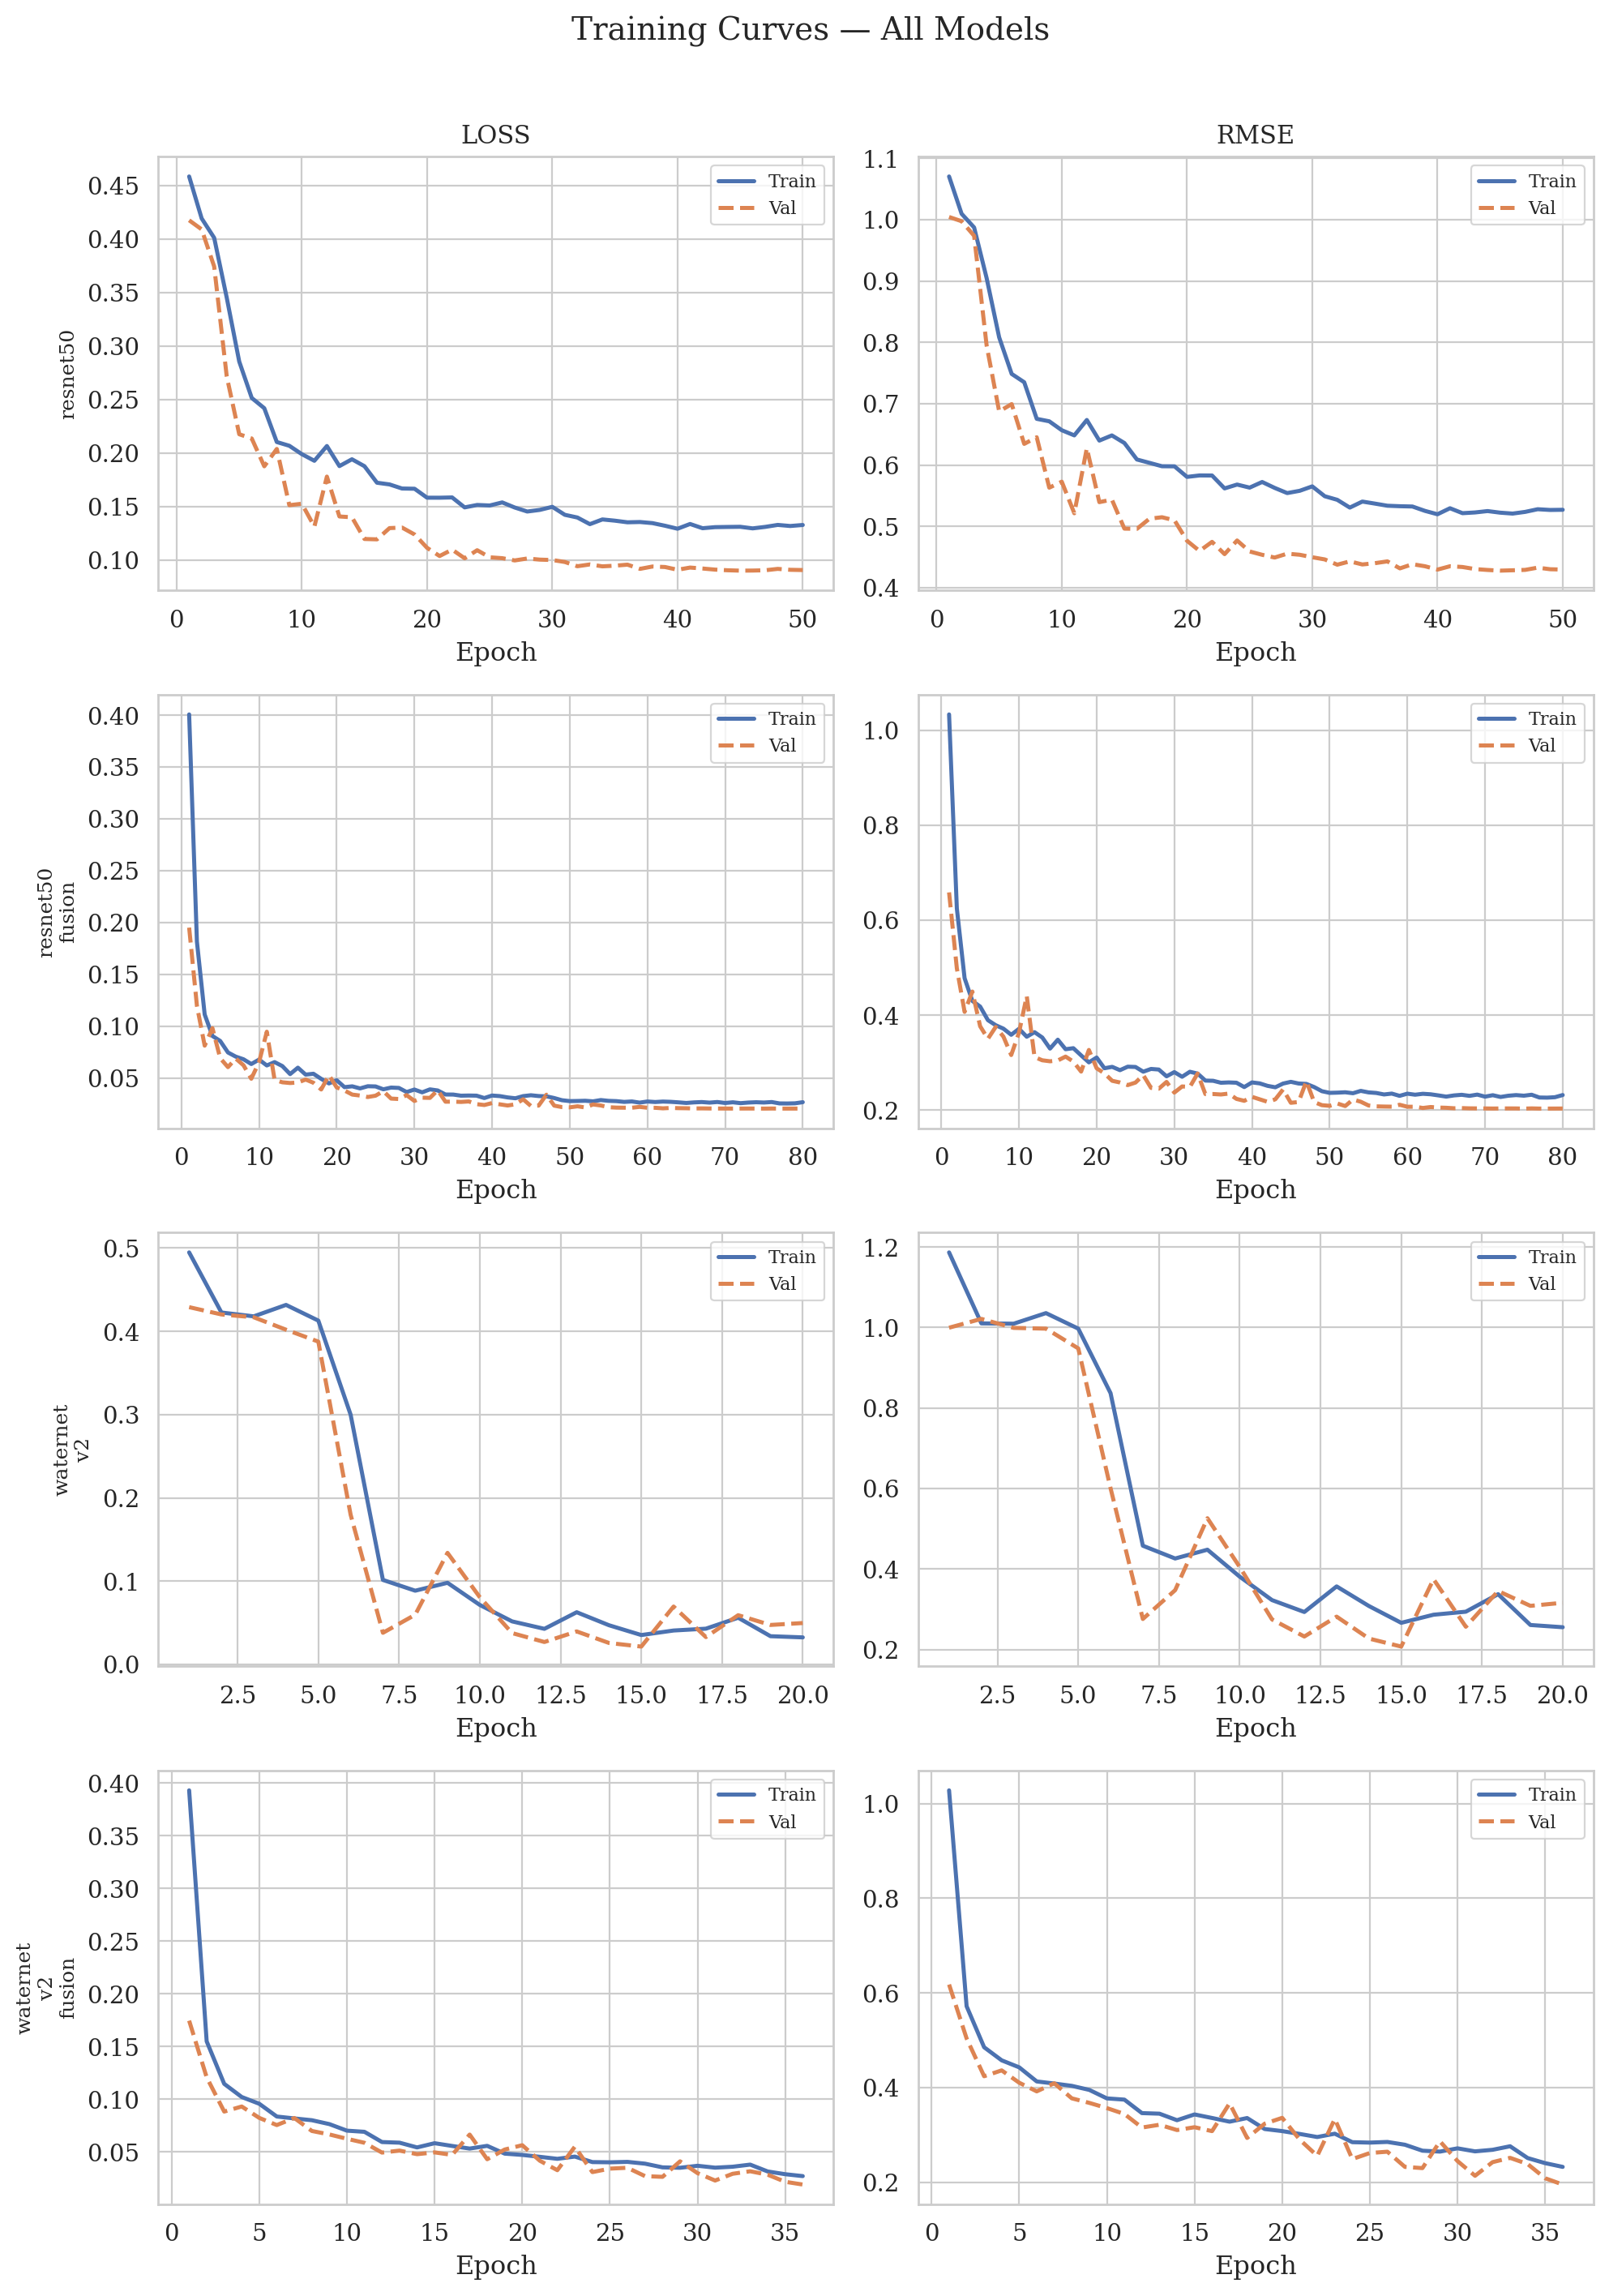
\includegraphics[width=\textwidth]{Images/training_curves.png}
    \caption{Training curves for all models, with loss and error function.}
    \label{fig:training_curves}
\end{figure}